\section{Conventional \ac{1D} datasets}
\label{sec:evaluation}

\subsection{``Twenty signals''}
\begin{sidewaysfigure}
    \centering
    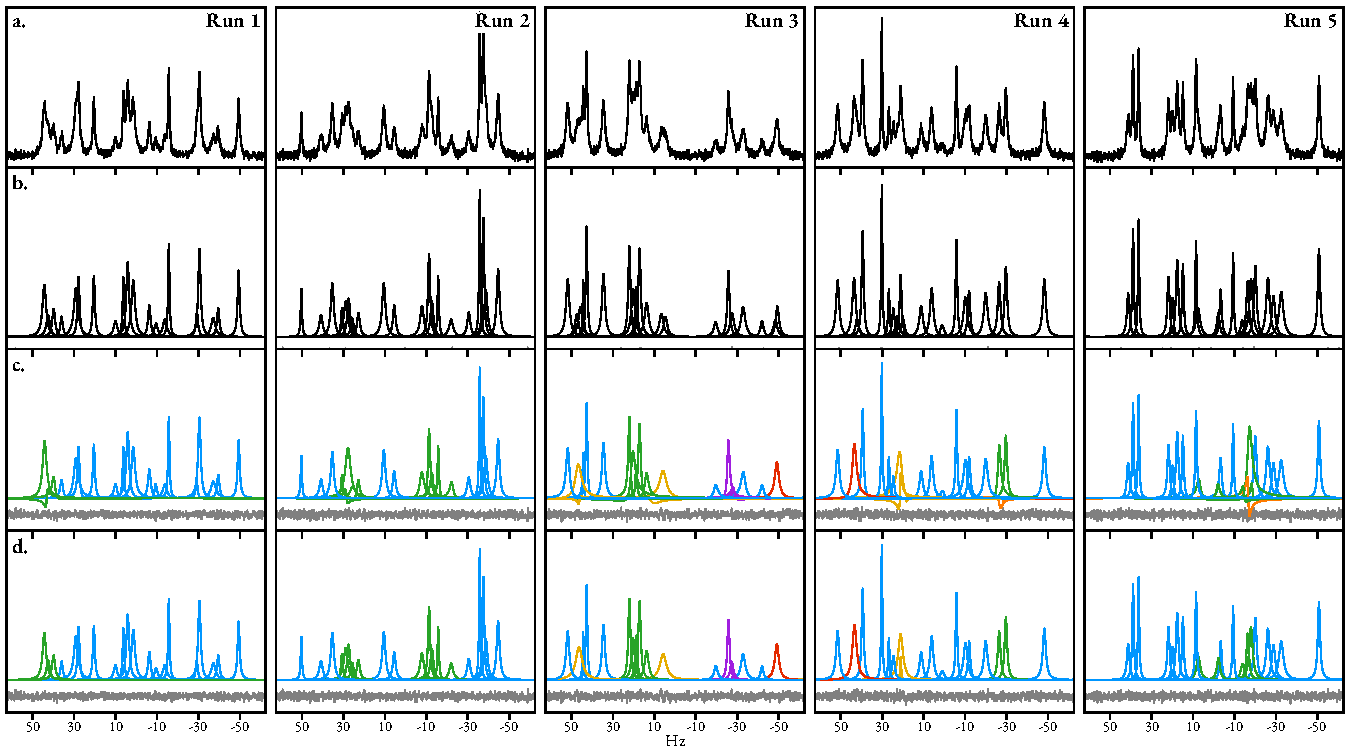
\includegraphics{mpm_vs_nlp/mpm_vs_nlp.pdf}
    \caption[
        The result of estimating a series of 5 simulated signals comprising 20
        oscillators, using solely the \acs{MPM} and also with phase
        variance-regularised \acs{NLP} afterwards.
    ]{
        The result of estimating a series of 5 simulated signals comprising 20
        oscillators (see the main text for details on how the datasets were constructed).
        \textbf{a.} Spectra of the datasets generated.
        \textbf{b.} Spectral lines corresponding to the true set of oscillators
        used to generate each dataset.
        \textbf{c.} Plots of spectral lines for each oscillator generated using
        the \acs{MPM}.
        \textbf{d.} An equivalent plot for the result after applying \acs{NLP},
        with the \acs{MPM} result being the initial guess.
        Also included in \textbf{c.} and \textbf{d.} is the residual between the
        data and the sum of the oscillator peaks (grey line).
        The colouring of oscillator lines in \textbf{c.} and \textbf{d.} is
        described in the main text.
    }
    \label{fig:mpm_vs_nlp}
\end{sidewaysfigure}
In order to assess the estimation routine proposed in \cref{chap:theory}
-- specifically the effectiveness of applying \ac{NLP} using an initial guess
generated using the \ac{MPM} -- a series of synthetic \acp{FID} were constructed
using \cref{eq:hypercomplex-fid} with $D=1$. For each \ac{FID}, a model order
of $M=20$ was used, the number of points sampled was $N = 1024$, the sweep
width was $\fsw=\qty{125}{\hertz}$, and the transmitter offset was $\foff
= \qty{0}{\hertz}$.  Each oscillator was assigned a phase of \ang{0}, while the
amplitudes, frequencies and damping factors were drawn at random from the
following distributions:
$a_m \sim \mathcal{U}(1, 5)$, $f_m \sim \mathcal{U}(\qty{-55}{\hertz},
\qty{55}{\hertz})$, $\eta_m \sim \mathcal{U}(\qty{2}{\per\second},
\qty{8}{\per\second})\ \forall m \in \lbrace 0, \cdots, 19\rbrace$. An extra
constraint was applied to the frequencies,
such that no two oscillators were permitted to have frequencies that differed
by less than $\nicefrac{4 \fswone}{\None} \approx \qty{0.49}{\hertz}$. Each
noiseless \ac{FID} $\bx$ was then corrupted with \ac{AWGN}, with a target
\ac{SNR} of \qty{25}{\deci\bel}, with the noise variance for each signal
determined using the equation
\begin{equation}
    \sigma^2 = \frac{1}{20^{2.5} N}
        \sum_{n=0}^{N-1} \lvert x_n \rvert^2.
\end{equation}
\note{Reference that this is the lowest
SNR that the MPM considered to be effective}.
The spectra of the simulated
\acp{FID} are presented in panel a of \cref{fig:mpm_vs_nlp}, with the set
of true oscillator peaks in panel b.

For each \ac{FID}, the \ac{MPM} was performed, assuming that the model order is
30, constituting a considerable over-fit. The \ac{MDL} tended to produce
considerable under-estimates of $M$ when applied to these \acp{FID}, so the
hard-coded value was used instead. Simulated signals featuring \ac{AWGN}
typically show a clean division between signal and noise components, with noise
components commonly being characterised by small amplitudes and/or very small
damping factors. For this reason, prior to subjecting the \ac{MPM} result to
\ac{NLP}, oscillators which satisfied either $a_m < 0.1$ or  $\eta_m <
\qty{0.7}{\per\second}$ were removed from the parameter set. The individual
oscillators which make up the \ac{MPM} result after purging spurious components
are displayed in panel c of \cref{fig:mpm_vs_nlp}, along with the
residual between the data and the summation of all the oscillator peaks.

The \ac{MPM} invariably generates a model with good agreement with the data, as
evidenced by the residual.
However, it can be seen that in several spectral regions across the datasets,
especially ones that are highly crowded, oscillators possess parameters which
deviate significantly from the true parameters, with the most notable feature
being individual oscillator phases -- these regularly stray far from \ang{0} --
and their associated amplitudes. The central motivation behind employing phase
variance-regularised \ac{NLP} is as a means of attempting to overcome this
detrimental feature of the \ac{MPM}.
In panel c of \cref{fig:mpm_vs_nlp}, the blue oscillators are those which
agree very closely with a particular oscillator in the true set of parameters.
Oscillators with other colours are not clearly mapped to a true oscillator,
with the different colourings described shortly.
The intention is for the \ac{NLP} routine to adjust the parameters describing
the non-blue oscillators in panel c such that they agree with oscillators found
in the true set, while not affecting the blue oscillators.
The results of \ac{NLP} at convergence ($\epsilon = \num{1e-8}$) are provided
in panel d.

In discussing the outcome of the routine, it will be useful to introduce the
concept of a \emph{frequency neighbourhood}, a loose term which describes a
small, continuous range of frequencies within the spectral window. As the
\ac{NLP} routine involves taking small steps
through parameter space in an attempt to converge, it is unlikely that an
oscillator which starts off with a frequency far away from a particular
frequency neighbourhood will eventually enter it.  As such, in order for the
\ac{NLP} routine to successfully estimate the region, sufficient oscillators
need to present within the neighbourhood in the first place. Cases where the
\ac{MPM} generated enough oscillators for a given frequency neighbourhood,
albeit with parameters which are noticeably off the true parameters are in
either green or yellow. Green oscillators are those which the \ac{NLP} routine
was able to adjust in order to achieve agreement with the true result. As such,
they indicate improvements to the estimation result as opposed to the \ac{MPM}
being used by itself. Conversely, yellow oscillators denote cases where, though
sufficient oscillators exist in the frequency neighbourhood in the initial
guess, the \ac{NLP} routine evolves such that at least one of the oscillators
is driven by the phase variance constraint to acquire a negative amplitude,
leading to it being purged from the parameter set. This typically occurs when an
oscillator has an initial phase which is considerably greater than \ang{90}.
Yellow oscillators therefore indicate cases where the final result has
under-fit the dataset. There are a few instances, denoted by red oscillators,
where the \ac{MPM} assigned too few oscillators to a particular frequency
neighbourhood, and as such the \ac{NLP} would not have been able to yield any
improvement.
The final two oscillator groupings, denoted by purple and orange, denote cases
where the \ac{MPM} generated more oscillators than are present in a given
frequency neighbourhood (i.e. the data was over-fit in this region). Orange
oscillators we purged by the \ac{NLP} routine due to their acquiring negative
amplitudes. This enabled a parsimonious fit of the frequency neighbourhood by
the oscillators which remained. Finally, the purple oscillators denote the one
occasion where an over-fit occurred, and the model order was not successfully
reduced by the \ac{NLP} routine.

Overall, it can be seen that the inclusion of \ac{NLP} broadly improves the
output of the \ac{MPM}, where crowded regions often get assigned oscillators
with spurious complex amplitudes ($a$ and  $\phi$). \note{More discussion here...}

\subsection{Andrographolide}
\begin{sidewaysfigure}
    \centering
    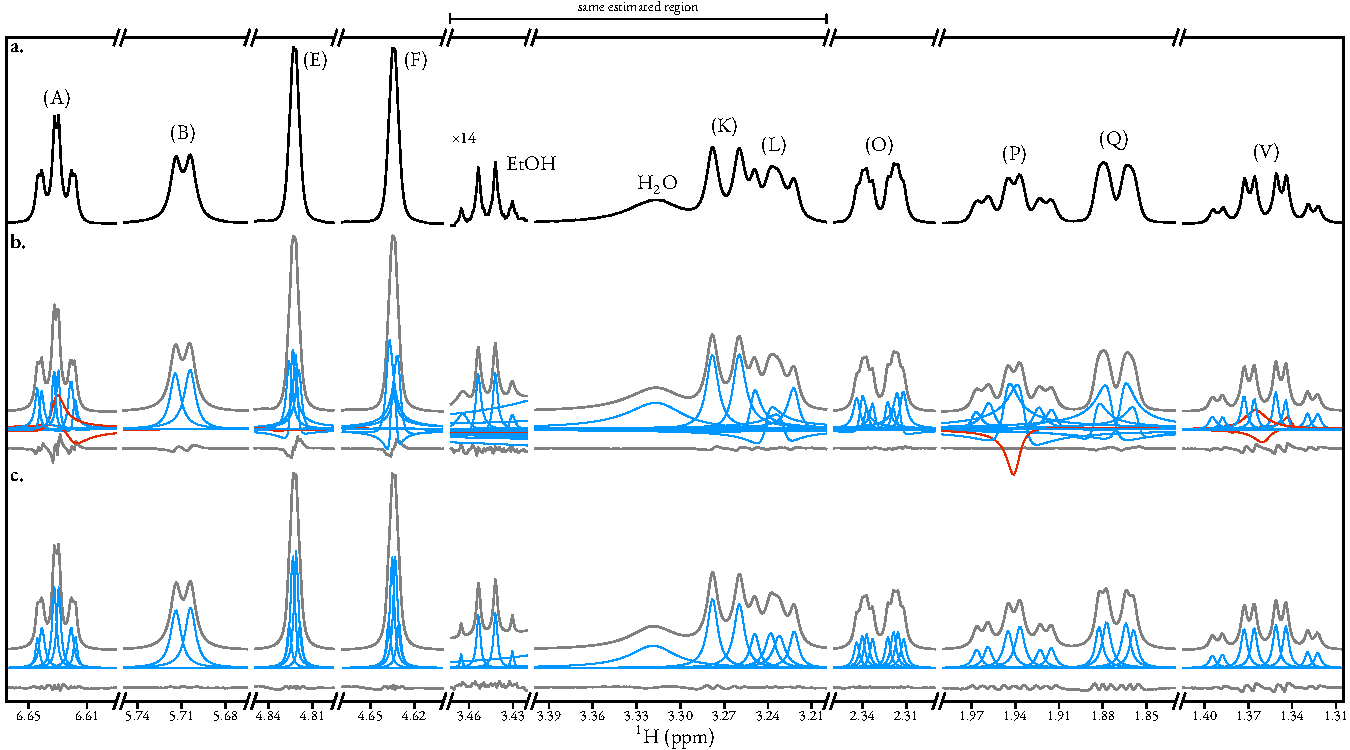
\includegraphics{andrographolide_onedim/andrographolide_onedim.pdf}
    \caption[
        Result of applying the estimation routine to selected regions of a
        pulse-acquire dataset of andrographolide.
    ]{
        Result of applying the estimation routine to selected regions of a
        pulse-acquire dataset of andrographolide in \acs{DMSOd6}.
        \textbf{a.} Spectral data corresponding to the regions considered.
        \textbf{b.} The result of applying the \acs{MPM} to the regions, with
        the model order predicted with the \acs{MDL}. Blue/red lines: peaks of
        individual oscillators, grey line above: the model (sum of all
        oscillators), grep line below: the residual between the data and the model.
        \textbf{c.} The result after convergence of the \acs{NLP} routine, again
        with the model above and residual below.
        Red peaks in panel b correspond to oscillators which acquire negative
        amplitudes during the \acs{NLP} routine, and are subsequently purged.
        Note that one of the reasons estimated has been split in two in the
        figure to save space, with one half, featuring a signal from ethanol,
        being magnified.
    }
    \label{fig:andro-onedim}
\end{sidewaysfigure}
\Cref{fig:andro-onedim} illustrates the outcome of applying the
estimation routine to selected regions of a \textsuperscript{1}H dataset of
andrographolide (\cref{fig:structures}.e) in \acs{DMSOd6} acquired with
a \qty{600}{\mega\hertz} spectrometer. The \ac{NLP}
routine is effective at resolving the spurious phase-behaviour often generated
by the \ac{MPM} (cf. panels b and c).
It's ability to estimate parameters from resonances with high
dynamic range and high variation of damping factors is also evidenced by the
fact that it was able to assign an intense broad singlet, corresponding to
water which has entered the sample over time, alongside a nearby quartet
corresponding to the methylene of some residual ethanol in the sample.

The routine generally does well at generating oscillators which describe the
apparent multiplet structures associated with each spin.
\Cref{tab:andro-multiplets} provides an overview of the most significant
couplings associated with the spins giving rise to the multiplet structures
considered.
\begin{table}
\centering
\begin{tabular}{c c c}
\hline
Spin  & Coupling partners & Multiplet structure \\
\hline
\multicolumn{3}{c}{\textbf{Andrographolide}}\\
\hline
(A) & (D)\textsuperscript{long}, (M)\textsuperscript{vic}, (N)\textsuperscript{vic} & ddd (\emph{dt}) \\
(B) & (D)\textsuperscript{ex} & d \\
(E) & (F)\textsuperscript{vinyl}, \dots & d\dots \\
(F) & (E)\textsuperscript{vinyl}, \dots & d\dots \\
(K) & (J)\textsuperscript{gem}, (H)\textsuperscript{ex} & d \\
(L) & (C)\textsuperscript{ex}, (T)\textsuperscript{180}, (U)\textsuperscript{60} & dd \\
(O) & (P)\textsuperscript{gem}, (R)\textsuperscript{60}, (V)\textsuperscript{60} & ddd \\
(P) & (O)\textsuperscript{gem}, (R)\textsuperscript{60}, (V)\textsuperscript{180} & ddd (\emph{dt}) \\
(Q) & (M)\textsuperscript{vic}, (N)\textsuperscript{v}, \dots & dd\dots \\
(V) & (O)\textsuperscript{60}, (P)\textsuperscript{180}, (R)\textsuperscript{g}, (W)\textsuperscript{180} & dddd (\emph{dq}) \\
\hline
\multicolumn{3}{c}{\textbf{Cyclosporin A}}\\
\hline
(A) & diastereotopic pair on \textsuperscript{\textbeta}C & dd \\
(B) & ---''--- & dd \\
(C) & ---''--- \& amide proton & ddd (\emph{dt}) \\
(D) & proton on \textsuperscript{\textbeta}C \& amide proton & dd \\
(E) & methyl protons on \textsuperscript{\textbeta}C \& amide proton & dq \\
(F) & ---''--- & dq (\emph{quintet}) \\
\hline
\end{tabular}
\caption[
    Major coupling partners associated with spins in andrographolide whose
    signals are considered in \cref{fig:andro-onedim}.
]{
    Major coupling partners associated with spins in andrographolide and
    cyclosporin A whose
    signals are considered in \cref{fig:andro-onedim,fig:andro-onedim},
    respectively, along with the
    apparent multiplet structures that arise.
    For andrographolide,
    coupling partners are labelled as follows:
    \textsuperscript{vinyl} geminal coupling between two vinylic protons,
    \textsuperscript{ex} geminal coupling between two protons, in which one
    if bonded to an oxygen, leading to exchange decoupling,
    \textsuperscript{gem} geminal coupling,
    \textsuperscript{long} long-range coupling,
    \textsuperscript{vic} vicinal coupling,
    \textsuperscript{60} geminal coupling, with a fixed dihedral angle of \ang{60},
    \textsuperscript{180} geminal coupling, with a fixed dihedral angle of \ang{180}.
    All cyclosporin couplings of significance are geminal couplings.
    In cases where the observed multiplet structure is different to the true
    structure, the observed structure is is in brackets.
}
\label{tab:andro-multiplets}
\end{table}
One of the most challenging aspects of estimating \ac{NMR} signals is
the fact that data frequently contains individual resonances with incredibly
similar frequencies due to the effect of scalar couplings. Molecules
with fused ring systems such as andrographolide are prime examples of spin
systems which generate such datasets, as they tend to have very dense coupling
networks leading to complex multiplet structures. Also, fused systems often
exhibit appreciable long-range couplings (between spins separated by four or more bonds) alongside more prevalent two-bond (geminal) and three-bond (vicinal) couplings.

Take the multiplet structure from spin (Q) as an example.
This has separate vicinal couplings to the
diastereotopic protons (M) and (N), which are likely the greatest magnitude couplings
associated with (Q). If these were the only couplings, a doublet of doublets
(dd) structure would be expected, which is what has been generated by
the estimation routine (see panel c in the region of
\SIrange{1.85}{1.88}{\partspermillion}). However, a comparison of the data and
the model indicates that there is a clear discrepancy between the two,
evidenced by systematic ``wiggles'' in the residual. This feature hints at an
under-fit of the multiplet structure.
The \ac{MPM} generated oscillators with phases deviating far from \ang{0} in
order to achieve a good agreement with the data in a residual sense, though of
course such a set of oscillators is unrealistic for a well-phased \ac{FID}.
Long-range couplings with magnitudes that are large enough to influence the
appearance of (Q)'s multiplet structure are likely to be present, which leads
to a signal in which all contributing resonances are too poorly resolved to
realistically gleam any further meaningful information, at least at the field
strength used.

As a second illustration, the signal corresponding to spin (V) is also
under-fit, this time because the presence of a number of couplings of similar
magnitudes leads to resonances coalescing at roughly the same frequency. For
(V), a multiplet structure featuring 16 resonances forming in a ``dddd''
structure is expected, however 3 of the couplings are of similar magnitudes,
such that individual resonances coalesce to form what is apparently a quartet
of doublets (dq). The estimation routine was able to resolve this dq structure,
however the large wobbles in the residual again signal that under-fitting has
occurred, and each oscillator is in fact being used to fit two or more
resonances present in the \ac{FID}. Again, at the field strength used to
acquire the \ac{FID}, it is unlikely that an accurate resolution of all 16
oscillators by estimation is feasible.

The fit to spin (O)'s multiplet structure has a very flat residual, indicating
that under-fitting is unlikely. With three major couplings of
different magnitude, a ``ddd'' multiplet structure in which all 8 signals
are discernible exits. The \ac{NLP} routine has performed effectively in
taking the initial guess from the \ac{MPM}, featuring the correct number of
oscillators albeit though with spurious phases, and generating a well-phased
set of oscillators defining the ddd structure.

Spin (L) also has 3 major couplings, though only a
dd structure is apparent, which is what has been assigned by the estimation
routine. The small residual  also implies that an under-fit has not occurred,
even though a ddd structure would be anticipated at first glance. However, one
of the coupling partners is a labile hydroxyl proton, which rapidly undergoes
exchange with other protons on the sample\footnote{
    Protons which are plausible exchange partners include those associated with
    residual water and ethanol in the sample, and hydroxyl protons from other
    andrographolide molecules.
}. Chemical exchange at a sufficiently
high rate leads to a ``decoupling'' of the spins, such that the two resonances
associated with a doublet coalesce into a broad singlet\cite[Section
2.6.1.5]{Claridge2016}.

\note{Discussion of more challenging regions? Probably beyond the scope of the
routine without further user input/maybe just too difficult full stop?}

\subsection{Cyclosporin A}
\begin{figure}
    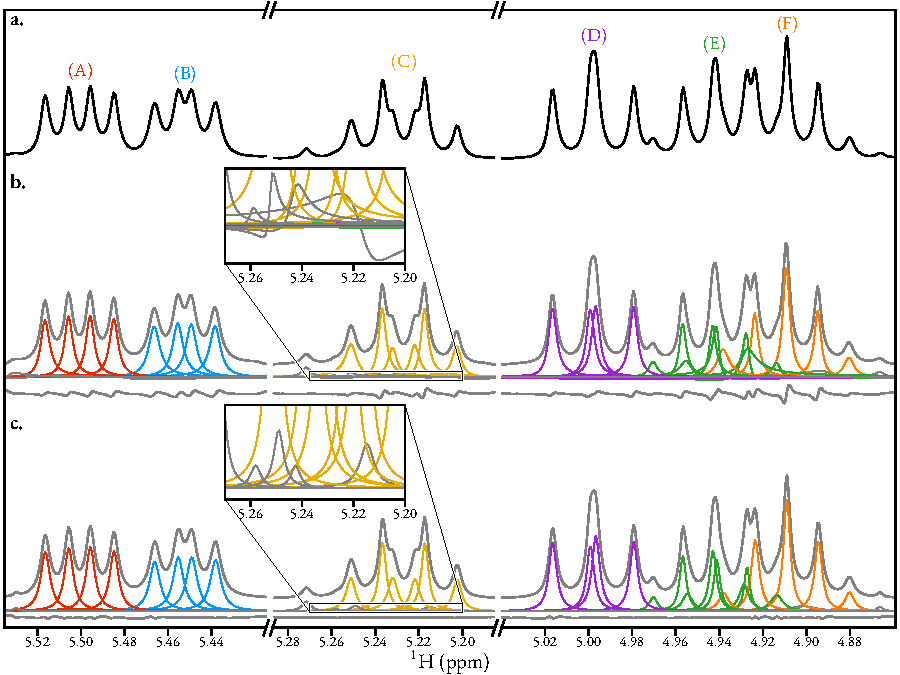
\includegraphics{cyclosporin/cyclosporin.pdf}
    \caption[
        Result of applying the estimation routine to selected regions of a
        pulse-acquire dataset of cyclosporin A.
    ]{
        Result of applying the estimation routine to selected regions of a
        pulse-acquire dataset of cyclosporin A in benzene-d\textsubscript{6}.
        The figure is of a similar layout to \cref{fig:andro-onedim}.
        Coloured peaks correspond to oscillators which have been assigned
        to multiplet structures of known spins. Grey oscillators correspond to
        those with an unknown association to a particular spin.
    }
    \label{fig:cyclosporin}
\end{figure}
The estimation routine was applied to regions of a \proton\ pulse-acquire
experiment of cyclosporin A \note{Structure in appendix}\,---\, a cyclic
peptide comprising 11 amino acids\,---\,in benzene-d\textsubscript{6}. The
regions considered all contain signals caused by protons bound to
C\textsuperscript{\textalpha} atoms in the peptide backbone\cite{Verma2018}.
Particular challenges in estimating this dataset are (a) the presence of
heavily overlapping signals, and (b) the presence of low intensity ``nuisance''
peaks, likely from impurities in the sample. Nevertheless, the routine has performed
effectively in generating a parameter estimate which agrees with the multiplet
structures present.

